\section{Experiments}
\label{sec:experiments}
In the following we briefly describe our experiment for visualizing the real large clinical data for the validation of the proposed approach. Then we describe the details of the evaluation and some heuristic tricks to improve the visualization result.
\subsection{dMRI and tractography segmentation}
Diffusion MRI (dMRI) data allow to reconstruct the $3D$ pathways of axons within the white matter of the brain as a set of
streamlines, called tractography. A streamline is a vectorial representation of thousands of neuronal axons expressing structural
connectivity. Recently, reconstruction and tracking algorithms~\cite{mori2002fiber,zhang2008identifying} allow to reconstruc the tractography from dMRI data. Our experiment is motivated by a clinical research hypothesis about the characterisation of the amiotrophic (ALS) disease, which is known to be affected by the corticospinal tract (CST)~\cite{cosottini2010evaluation,sage2009quantitative}. The first task is to segment the CTS from the full brain tractography. 

Let the polyline $s =\{ \vec{x_1},\ldots,\vec{x}_{n_s}\}$, where $\vec{x} \in \mathbb{R}^3$, be a \emph{streamline} reconstructed from dMRI data by deterministic tractography algorithms~\cite{mori2002fiber}. Let the \emph{tractography} $ \mathbb{T}  = \{s_1,\ldots,s_N\}$ be defined as a set of $n$ streamlines, for which $N \sim 3 \times 10^5$ usually. Let $d:\mathcal{X} \times
\mathcal{X} \mapsto \mathbb{R}^+$ be a distance function between
streamlines. A common distance between streamlines is the symmetric
minimum average distance (see~\cite{zhang2008identifying}) defined as
$d(X_a,X_b) = \frac{1}{2}(\delta(X_a,X_b) + \delta(X_b,X_a))$ where
\begin{equation}
  \label{equ:mam_distance}
  \delta(X_a,X_b) = \frac{1}{|X_a|} \sum_{\mathbf{x}_i \in X_a}
    \min_{\mathbf{y} \in X_b} ||\mathbf{x}_i - \mathbf{y}||_2.
\end{equation}
Inspite that recently there is an increasing literature in automatic
segmentation using machine learning techniques (see a brief review in~\cite{wang2011tractography,olivetti2011supervised}), applications in the
clinical domain rely on manual segmentation. The manual segmentation process consumes a lot of time and effort due to the large number of streamlines, in the order of $3 \times 10^5$, which make it intrinsically difficult both to inspect and to unfold the anatomical structures. Morover, 
%a lengthy and complex task for two reasons: first the tractography is a very large set of reconstructed neuronal pathways, 
%(see Figure~\ref{fig}). Second, 
it is claimed that there is a lack of software tools to support and to simply this segmentation process~\cite{olivetti2012fast}. In this experiment, we conceive a novel computer-assisted interactive process based on the meothod of multiple scale for representation the large tractography described in section~\ref{sec:methods}.
\paragraph*{ALS dataset:}
the data we used in this expermient is recorded with a $3T$ scanner at Utah Brain Institute. It
consisted the recordings of $12$ ALS patients and $12$ healthy
controls; $64$ ($+1$, i.e. $b=0$) gradients; $b$-value$=1000$.;
anatomical scan ($1 \times 1 \times 1mm^3$).  We reconstruct the
streamlines using EuDX, a deterministic tracking algorithm
~\cite{garyfallidis2012towards} from the DiPy
library~\footnote{\url{http://www.dipy.org}}. % We just present results on one subject.
\paragraph*{The dissimilarity representation: }
%\emph{cut and paste from PRNI2013 - need to repharse}
Due to the fact that most of the state-of-the-art learning techniques often require the data to lie in a vectorial space, which is not the case of streamlines, which has different length and different number of points. And for this reason they cannot be directly represented in a common vectorial. In this case, we need to find a representation $\phi$ of streamline in a vectorial space, by mapping a streamline $s$ from its original space $\mathbb{T}$ to a vector of $\mathbb{R}^d$ - $\phi : \mathbb{T} \mapsto \mathbb{R}^d$, where $d$ is the dimension of the new space. One suggestion for this is the \emph{dissimilarity representation}~\cite{pekalska2002generalized}. It is a lossy Euclidean embedding algorithm was previously proposed
in~\cite{olivetti2012approximation} for streamlines. The dissimilarity representation
is defined as $\phi_{\Pi}^d(X):\mathcal{X} \mapsto \mathbb{R}^p$ s.t.
\begin{equation}
  \phi_{\Pi}^d(X) = [d(X,\tilde{X}_1) ,\ldots, d(X,\tilde{X}_p)]
\label{equ:dissimilarity_representation}
\end{equation}
where $d$ is a distance function between streamlines, and $\Pi =
\{\tilde{X}_1, \ldots, \tilde{X}_p\} \subset \mathcal{X}$ is a set of
$p$ streamlines called \emph{prototypes}. The quality of the Euclidean
embedding is strongly dependent on the selection of the prototypes
(see~\cite{pekalska2006prototype,olivetti2012approximation}). More detail can be found in ~\cite{olivetti2012approximation}.
%An efficient procedure to select effective prototypes in the case of tractography data was presented in~\cite{olivetti2012approximation}: the \emph{subset farthest first} (SFF) algorithm. This procedure is a stochastic and scalable version of the farthest first traversal (FFT) algorithm which is a standard greedy solution to the well known $k$ centre problem. This problem, put in our context, entails selecting a set $\Pi$ of $p$ streamlines~\footnote{Note that here we use $p$ to denote the size of $\Pi$ instead of the $k$ of the ``$k$ centre problem''. This is to avoid confusion with the notation we adopt in this paper.} such that the sum of the distances of each streamline of the tractography to closest streamline in $\Pi$ is minimised.
% Intuitively the streamlines in $\Pi$ are designed to be a % \emph{representative} sample of the whole tractography.
%%The FFT algorithm selects one streamline at random from the tractography as the first prototype $\tilde{X}_1$ and then iteratively adds a new prototype as the one maximising the distance to the already selected prototypes. The SFF algorithms is a stochastic scalable version of FFT, which subsamples $m = \lceil c p \log p \rceil$ streamlines from the whole tractography, and then applies FFT to the subsample. For the case of tractography data, when $c>=3$ the SFF algorithm is comparable to the FFT algorithm with high probability, following the proof in~\cite{turnbull2005fast} and the empirical results in~\cite{olivetti2012approximation}.
By applying the hieararchical clustering algorithm (section~\ref{subsec:hierarchical}) on the dissimilarity approximation, the hierarchical tree $\mathcal{H}$ could be created.
\subsection{Multiple scales for representation}
\paragraph{Scale measurement: }
As the measurement for computing the level of detail of a cluter $s(C)$, we use the height of the cluster $C$ within the hierarchical tree $\mathcal{H}$. The reason is that it leads to continuous and thus provides smooth transitions on our hierarchical display. Choosing the height of cluster as the measurement for the level of detail, together with a proper interactive tool to support roll up (down) operations, the visualization can be explored at different levels of abstraction easily. 

Let $h$ be the height of hierarchical tree $\mathcal{H}$: $h = height(\mathcal{H})$, At the leaf $C_{leaf}$ of $\mathcal{H}$, the heigh is in the order of zero, thus $s_{min} = 0$. In the similar way, $s_{max} = 1$ becasue at the root $C_{root}$ of the tree $\mathcal{H}$, $heigh(C_{root} = h$.  The range scale of $\mathcal{H}$ is $[s_{min}, s_{max}] = [0,1]$, and $\forall C_i \in \mathcal{H}, s(C_i) = \frac{height(C_i)}{h}$, where $heigh(C_i)$ is the heigh of the cluster $C_i$~\cite{yang2003interactive}. Intuitively, this measurement satisfies the condition of definition of the level of detail in~\ref{def:level_detail}, because if $C_i$ is an ancestor of $C_j$, then $heigh(C_i) \geq heigh(C_j)$ and thus, $s(C_i) \geq s(C_j)$
%s = [0,1], where 0 is the whole leaves (streamlines) and 1 is the only one root. Scale s can be defined based on the height of tree h: 0/h, 1/h, ..., (h-1)/h, h/h; or the maximum distance of each node of the tree \cite{yang2003interactive}
%\paragraph{Choosing multiple scales for representation}

By looking at the local maxima of the goodness score as definition in~\ref{def:goodness_scale}, we can estimate the most relevant scale factores for representing the tree $\mathcal{H}$, and thus getting the multiple scale representation $\mathsf{\textit{B}} = \{b_1, b_2, \ldots, b_k\}$. The figure~\ref{fig:goodness_score} shows a visualization of two goodness scores of subject $1$(left) and subject $2$(right) from ALS dataset. 
%Focusing on the local maxima value of goodness score leads us to the meaningful scale factors for representing the tree $\mathcal{H}$. 
For example with subject $109$ (left) the multiple scale representation $\mathsf{\textit{B}}_{1}$ could be concluded as $\mathsf{\textit{B}}_{1} = \{\frac{8}{h_1}, \frac{10}{h_1}, \frac{12}{h_1}, \frac{18}{h_1}, \frac{22}{h_1},\frac{25}{h_1},\frac{27}{h_1}, \frac{18}{h_1}\}$, where $h_1$ is the heigh of the hierarchical tree of subject $1$: $h_1= height(\mathcal{H}_{1})$; Similarly, with subject $20$, $\mathsf{\textit{B}}_{2} = \{\frac{10}{h_2}, \frac{16}{h_2}, \frac{19}{h_1}, \frac{24}{h_2},\frac{27}{h_2}\}$, where $h_2= height(\mathcal{H}_{2})$. Taking into account that $b_i$ should be chosen from the small scale factor to the large one in order to satifies the condititon of an ordered set in the definition~\ref{def:multi_scales_representation}, of which the underlying idea is to make sure a continuos and smooth order of visulaization when users switch among these levels. This experiment exame the ability of our proposed method to compute the multiple scales representation for a large data. Note that we just present two sample of results here, we also run on other subjects and get the multiple scale representation for each of them.
\begin{figure}
  \centering
  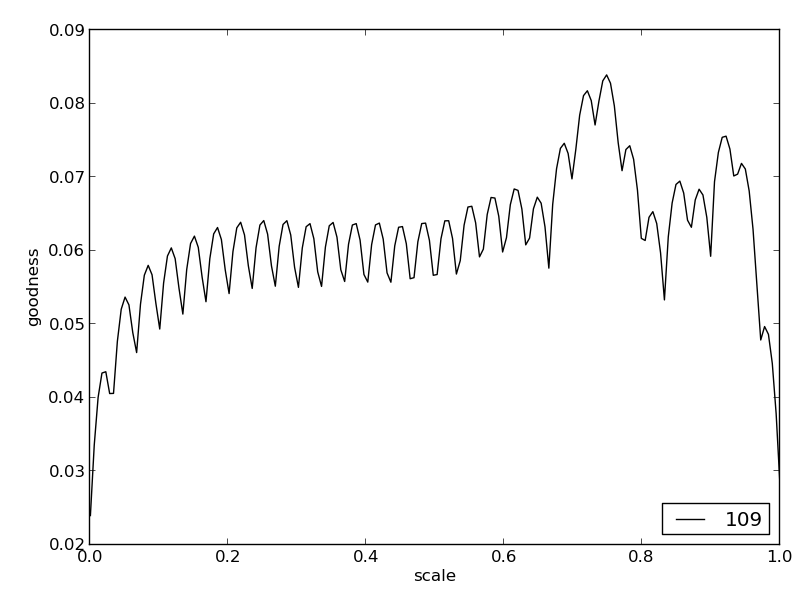
\includegraphics[width=6.0cm]{109_goodness_R_function.png}
  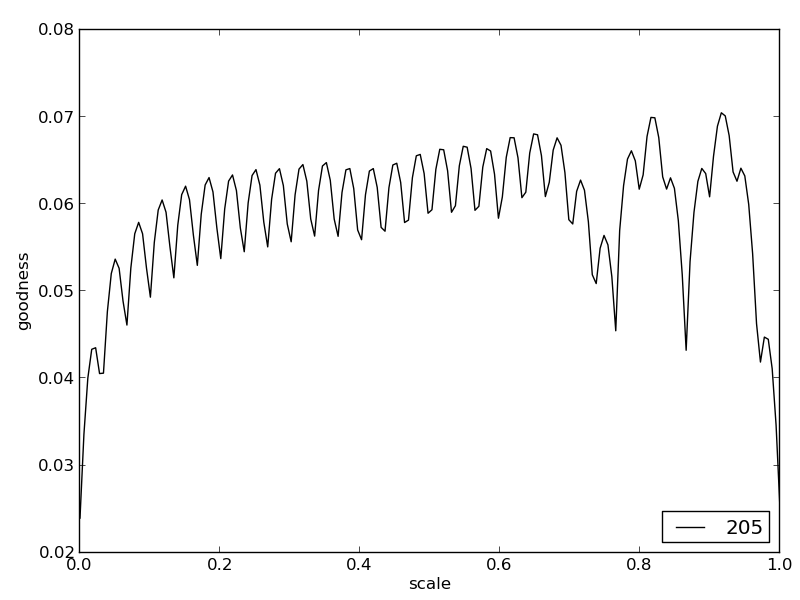
\includegraphics[width=6.0cm]{205_goodness_R_function.png}
  \caption{Goodness score of subject 109 and 205 from ALS dataset}% at different scale factor}
  \label{fig:goodness_score}
\end{figure}
%\paragraph*{Evaluate the multi scale representation}
We are now in the state of being ready to evaluate the multiple scale representation $\mathsf{\textit{B}} = \{b_1, b_2, \ldots, b_k\}$. Based on the definition~\ref{def:best_scales} about the goodnes of a scale factor $b \in \mathsf{\textit{B}}$, we implemented a program as the peusdo code in~\ref{alg:evaluate} with $\lambda_1 = 15$ and $\lambda_2=50$. In figure~\ref{fig:goodness_score} - left, we plot the mean goodness score of each multiple scale representation for five subjects from ALS dataset, together the standard derivation for $20$ iterations. Note that on the horizontal axis, the cut scales $k$ represented on this figure is the index of the coresponding real scale $\frac{k}{h}$. 
\begin{figure}
  \centering
  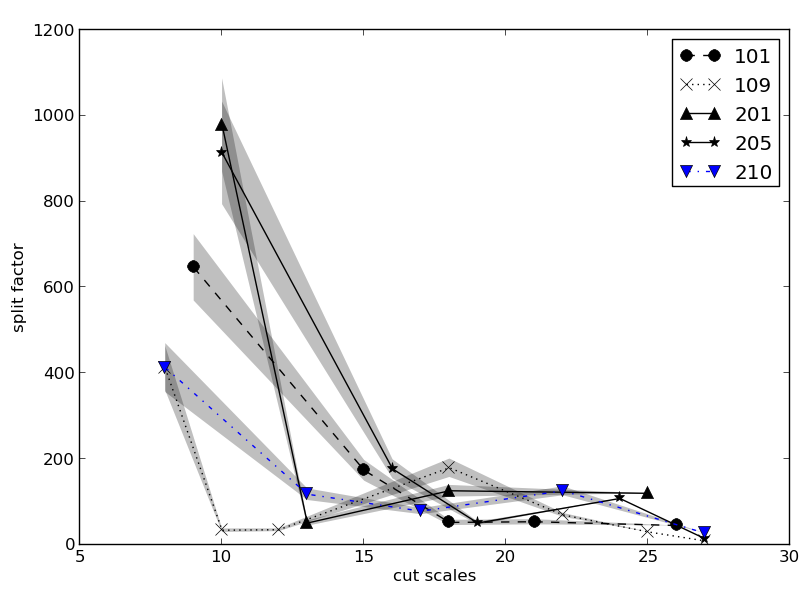
\includegraphics[width=6.0cm]{evaluate_cut_based_on_split_factor_130527.png}
  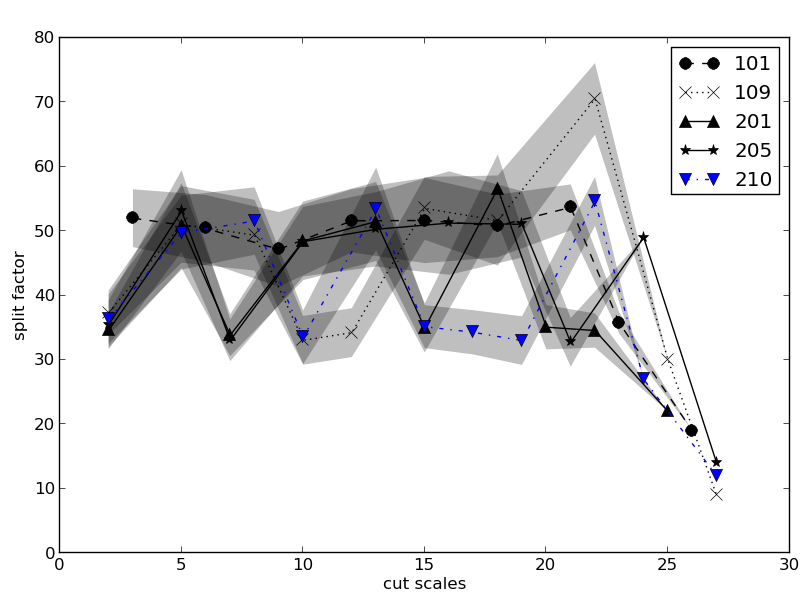
\includegraphics[width=6.0cm]{evaluate_cut_based_on_split_factor_130527_heuristic.png}
  \caption{Split factor before(left) and after(right) adding heuristic constrains}
  \label{fig:goodness_score}
\end{figure}

%\paragraph*{Heuristic for improving the multi scale representation}
Exept for the first chosen scale $b_1$, almost other scale $b_k \in \mathsf{\textit{B}}, k \neq 1$, the split factor $\xi(S_{(b_i,\lambda_1)},b_{i+1})$ satisfies the condition in equation~\ref{equ:best_scale}. Note that from the leaf (scale $0$) the goodness score increases linearly, reaches the peak at scale $B_1$, and then changes fluctuately. It means that the split factor of the cut at $b_1$ to the leaf (scale $0$), $\xi(S_{(b_1,\lambda_1)},0))$, is usually very large comparing with other split factor. However, in the point view of visualization, all the split factor $\xi(S_{(b_i,\lambda)},b_{i+1})$ should be around $\lambda_2$. Due to this, for the saking of better representation, we add an heuristic constrains to the chosen scale set that the distance between two closest chosen scale $b_i$ and $b_{i-1}$ should not exceed a threshold $\theta$: $d(b_i,b_{i-1}) \leq \theta$ (in the case of $b_1$, the distance with the leaf $d(b_1,0)$ is used). The results after adding this heuristic constrains is showed in the figure~\ref{fig:goodness_score} - right. 
These results, demonstrate that our proposed method of choosing multiple scales for visualization large data is efficiently and robust to the size of the data. 


